\documentclass{beamer}%Beamer is a LaTeX document class for creating slides for presentations.
\usetheme{metropolis}%


\usepackage{graphicx}%this package allows graphics inclusion
\usepackage{subcaption}
\usepackage[utf8]{inputenc}
\usepackage[spanish, mexico]{babel} %specify document language
%\usepackage[usenames, dvipsnames]{color}

\definecolor{pur}{RGB}{139,0,139}
\definecolor{ver}{RGB}{46,139,87}


\title{Base de Datos Avanzada}%Course name
\date{\today}%Can be set to a specific date with "2018 Agosto 08". "\date" must be used before "\maketitle"
\author{Edher Nu\~no \\ Miguel Ochoa} % \\ breaks the line
\institute{Universidad Aut\'onoma de Guadalajara}


\begin{document}
\maketitle %render title page

\section{Problem\'atica}

\begin{frame}{Problema}
Colecci\'on de peliculas con :
\begin{itemize}
\item Entradas repetidas sin control.
\item Pocas a nulas referencias para intercambio.
	\begin{itemize}	%on beamer "\subitem" can't be used, this is an alternative
		\item[a)] Estudio.
		\item[b)] Director.
	\end{itemize}	
\item Informaci\'on de parametros.
	\begin{itemize}
		\item[a)] Duraci\'on.
		\item[b)] Budget vs Revenue.
	\end{itemize}		
\end{itemize}
\end{frame}

\section{Dise\~no de la base de datos.}
\begin{frame}{Diagrama Entidad-Relaci\'on}
\centering
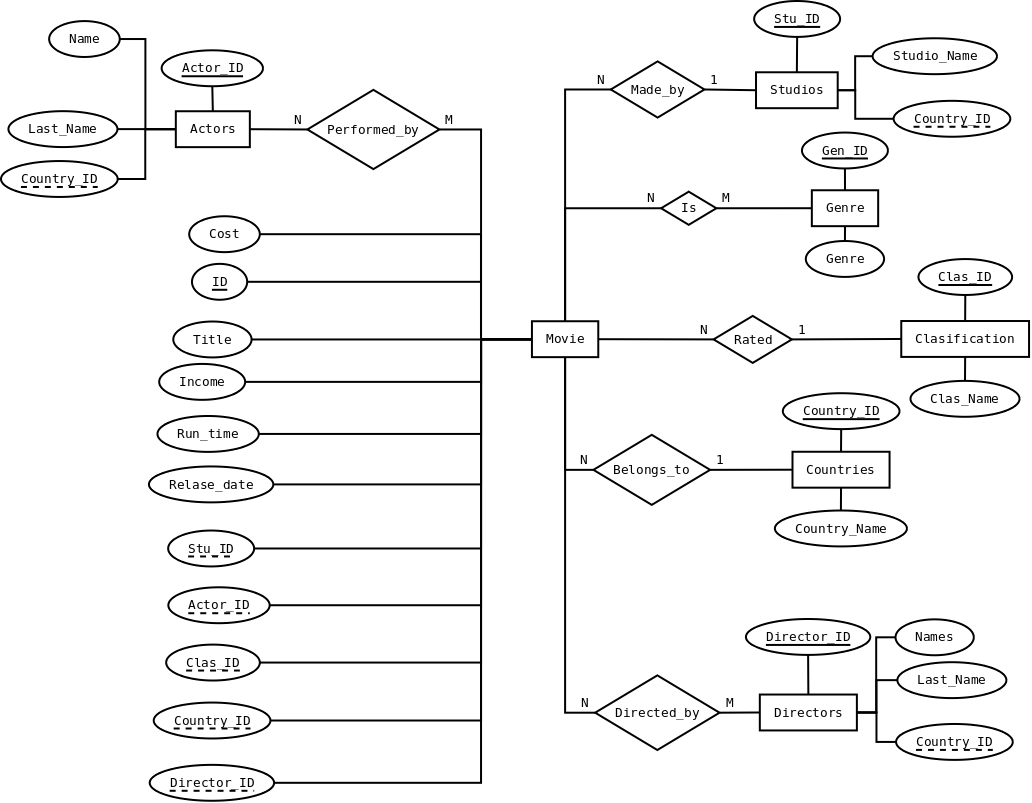
\includegraphics[scale=0.295]{figures/entidad_relacion_01.png}
\end{frame}

\section{Implementaci\'on}
\begin{frame}{Implementaci\'on}
\centering
\begin{tabular}{p{4cm}cp{4cm}}
\texttt{\textcolor{pur}{CREATE TABLE} COUNTRY (ID \textcolor{ver}{INTEGER} \textcolor{pur}{NOT NULL} GENERATED ALWAYS AS IDENTITY (START WITH 1 INCREMENT BY 1), NAME \textcolor{ver}{VARCHAR(30)} \textcolor{pur}{UNIQUE NOT NULL},
    PRIMARY KEY(ID)
);}

& \hspace{1cm} &
 Crea la tabla de paises con el campo ID como llave primaria y generada autom\'aticamente\\
\end{tabular}
\end{frame}

\begin{frame}{Implementaci\'on}
db2 LIST TABLES FOR SCHEMA MOVIEINDEX
\begin{center}
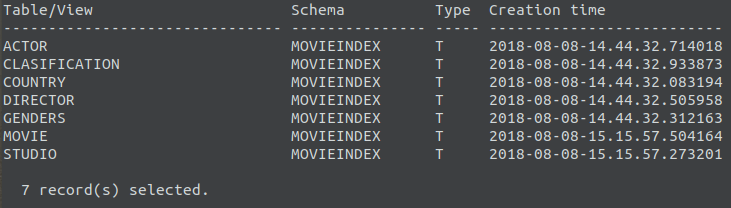
\includegraphics[scale=0.4]{figures/screenshot_output_list_tables.png}
\end{center}
\end{frame}

\begin{frame}{Implementaci\'on}
db2 DESCRIBE TABLE MOVIEINDEX.MOVIE
\begin{center}
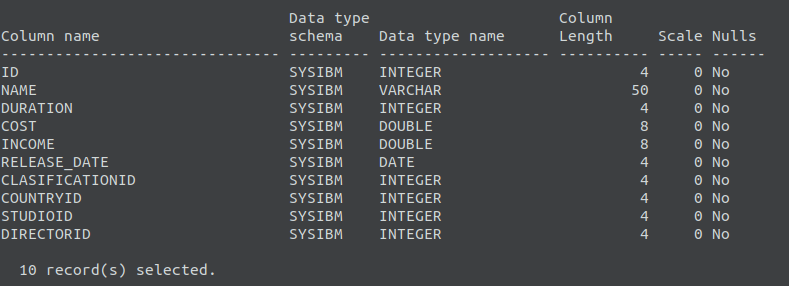
\includegraphics[scale=0.4]{figures/screenshot_output_movie_description.png}
\end{center}
\end{frame}


\begin{frame}{Tablas}
\begin{figure}
    \centering
    \begin{subfigure}[b]{0.3\textwidth}
        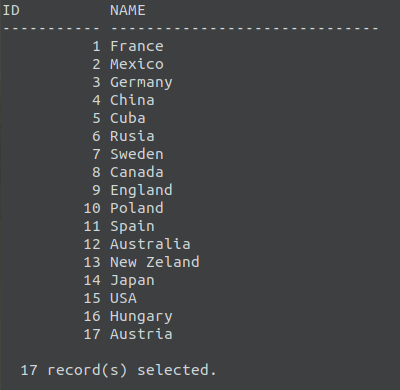
\includegraphics[scale=0.2]{figures/screenshot_country_data.png}
        \caption{Country Table}

    \end{subfigure}
    ~ %add desired spacing between images, e. g. ~, \quad, \qquad, \hfill etc. 
      %(or a blank line to force the subfigure onto a new line)
    \begin{subfigure}[b]{0.4\textwidth}
        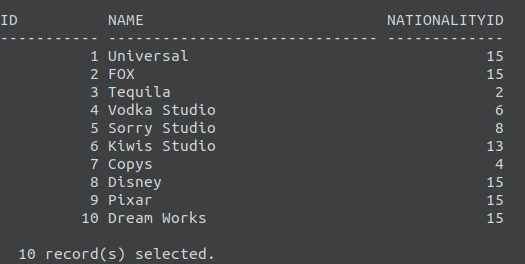
\includegraphics[scale=0.2]{figures/screenshot_studio_data.png}
        \caption{Studio Table}

    \end{subfigure}
    ~ %add desired spacing between images, e. g. ~, \quad, \qquad, \hfill etc. 
    %(or a blank line to force the subfigure onto a new line)
    \begin{subfigure}[b]{0.3\textwidth}
        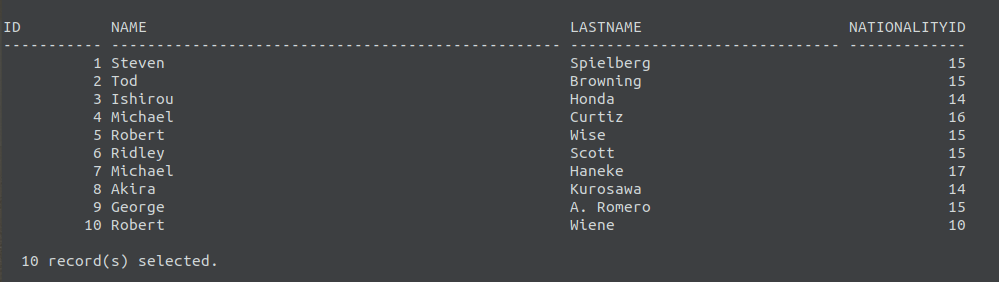
\includegraphics[scale=0.2]{figures/screenshot_director_data.png}
        \caption{Director Table}

    \end{subfigure}
    \caption{Tablas en la MOVIESDB parte 1}
\end{figure}
\end{frame}

\begin{frame}{Tablas}
\begin{figure}
    \centering
    \begin{subfigure}[b]{0.3\textwidth}
        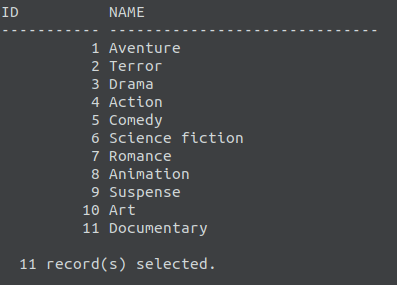
\includegraphics[scale=0.2]{figures/screenshot_gender_data.png}
        \caption{Gender Table}

    \end{subfigure}
    ~ %add desired spacing between images, e. g. ~, \quad, \qquad, \hfill etc. 
      %(or a blank line to force the subfigure onto a new line)
    \begin{subfigure}[b]{0.4\textwidth}
        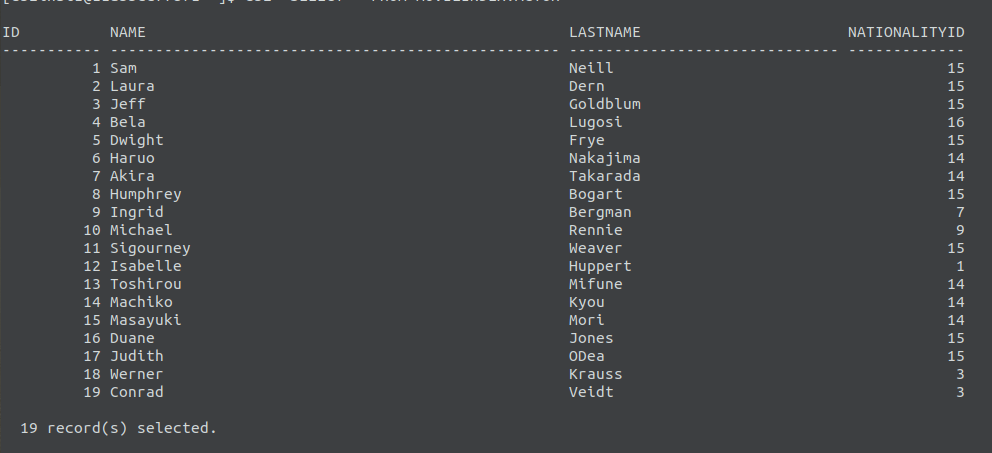
\includegraphics[scale=0.2]{figures/screenshot_actor_data.png}
        \caption{Actor Table}

    \end{subfigure}
    ~ %add desired spacing between images, e. g. ~, \quad, \qquad, \hfill etc. 
    %(or a blank line to force the subfigure onto a new line)
    \begin{subfigure}[b]{0.3\textwidth}
        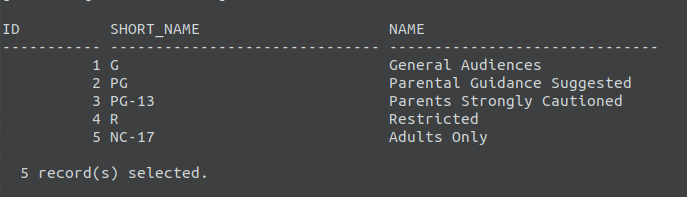
\includegraphics[scale=0.2]{figures/screenshot_clasification_data.png}
        \caption{Clasification Table}

    \end{subfigure}
    \caption{Tablas en la MOVIESDB parte 2}
\end{figure}
\end{frame}

\section{Vistas}
\begin{frame}{Vistas}
	\begin{figure}

		\begin{subfigure}[b]{1\textwidth}
			\begin{tabular}{|c|c|c|}\hline
				Country		&		Movie Name		&		Relase Date \\ \hline
				USA			&		Jurassic Park	&		1993-06-09	\\	\hline
				Japan		&		Rashomon		&		1950-08-25	\\	\hline
				$\cdot$ $\cdot$ $\cdot$		&	$\cdot$ $\cdot$ $\cdot$		& $\cdot$ $\cdot$ $\cdot$ \\ \hline
			\end{tabular}
			\caption{Vista: Peliculas por paises}
		\end{subfigure}
		
		\begin{subfigure}[b]{1\textwidth}
		\begin{scriptsize}
			\begin{tabular}{|p{0.1\textwidth}|p{0.1\textwidth}|p{0.1\textwidth}|p{0.1\textwidth}|p{0.1\textwidth}|p{0.1\textwidth}|p{0.1\textwidth}|p{0.1\textwidth}|}\hline


	Name	&	Duration	&	Cost	&	Income	&	Release Date	&	Clasification	&	Studio	&	Director	\\ \hline
Jurassic Park & 127 & \$63 Millones & \$920.1 Millones & 1993-06-09 &	PG-13 & Universal & Steven Spielberg\\ \hline
Jurassic Park & 127 & \$63 Millones & \$920.1 Millones & 1993-06-09 &	PG-13 & Universal & Steven Spielberg\\ \hline
$\cdot$ $\cdot$ $\cdot$		&	$\cdot$ $\cdot$ $\cdot$		& $\cdot$ $\cdot$ $\cdot$  &$\cdot$ $\cdot$ $\cdot$		&	$\cdot$ $\cdot$ $\cdot$		& $\cdot$ $\cdot$ $\cdot$ &$\cdot$ $\cdot$ $\cdot$		&	$\cdot$ $\cdot$ $\cdot$	\\ \hline
			\end{tabular}
		\end{scriptsize}
			\caption{vista1}
		\end{subfigure}		
	\end{figure}
	
\end{frame}
\begin{frame}{Vistas}
Para esta Base de Datos se implementaron 5 \textit{Vistas:}
\begin{itemize}
\item $COUNTRYID\_MOVIES:$ Permite ver las entradas de la tabla pelicula ordenadas en base al pa\'is de origen (alfab\'eticamente). El resultado de esta \textit{vista} se presenta en ejemplo en la figura \ref{vista1}.

\item $TOP\_INCOME\_MOVIES:$ Permite ver una lista de las 10 peliculas con mayores ingresos.

\item $LOWEST\_INCOME\_MOVIES:$ Permite ver una lista de las 10 peliculas con menores ingresos.
\end{itemize}
\end{frame}


\begin{frame}{Vistas}
\begin{itemize}
\item $TOP\_EXPENSIVE\_MOVIES$: Muestra todas las entradas de la tabla \textit{MOVIE} ordenadas por su costo.
\item $MOVIES\_REVENUES:$ Muestra una lista de las peliculas con mayores ganancias, un ejmplo de esta vista se muestra en la figura \ref{vista3}.
\end{itemize}
\end{frame}
	

\begin{frame}{Vistas}
\begin{figure}
    \centering
  	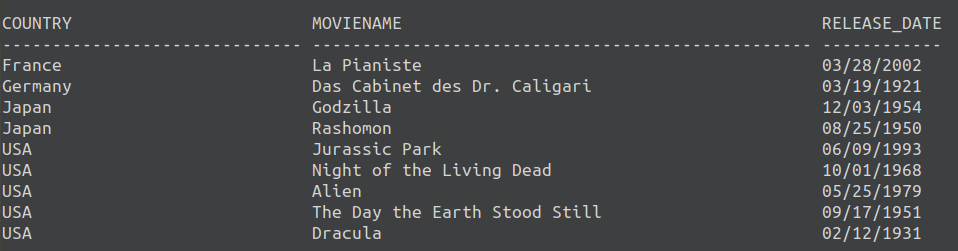
\includegraphics[scale=0.3]{figures/screenshot_vista1.png}
  	\caption{Vista de peliculas en base a su pa\'is de origen.} \label{vista1}
\end{figure}

\end{frame}

\begin{frame}{Vistas}
\begin{figure}
    \centering
  	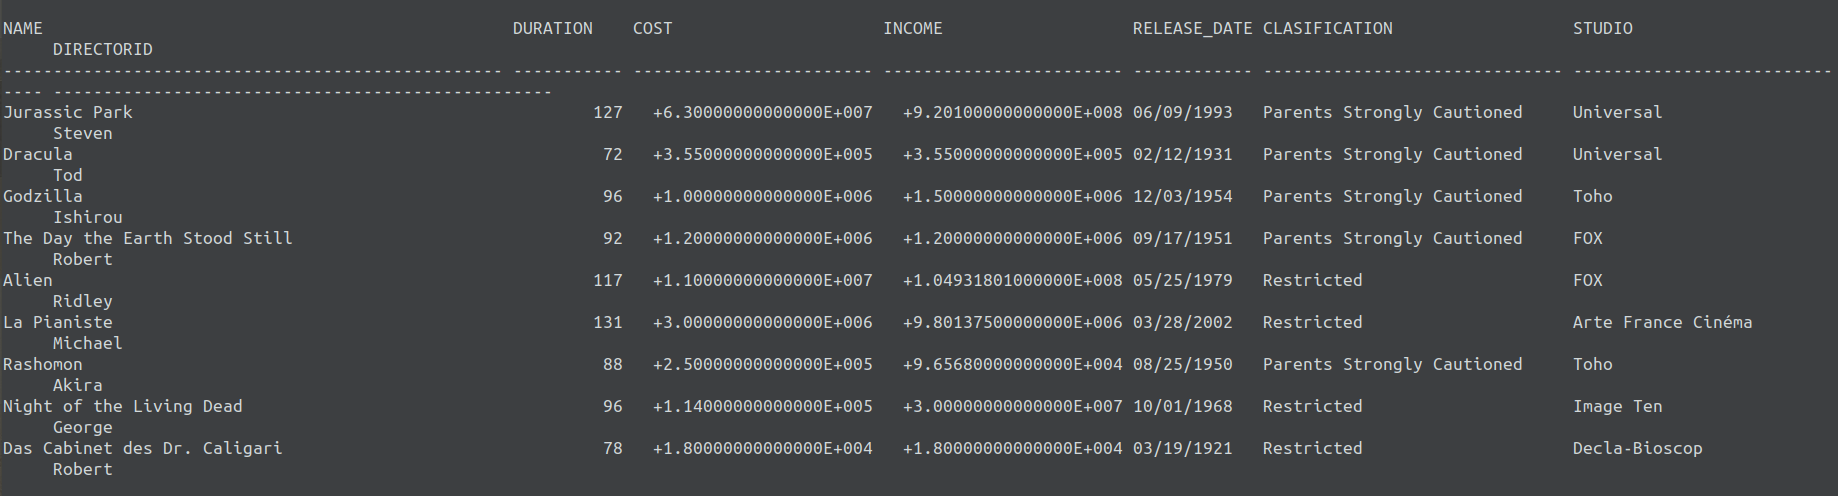
\includegraphics[scale=0.15]{figures/screenshot_vista2.png}
  	\caption{Vista de peliculas en base sus Recaudaciones.} \label{vista2}
\end{figure}
\end{frame}


\begin{frame}{Vistas}
\begin{figure}
    \centering
  	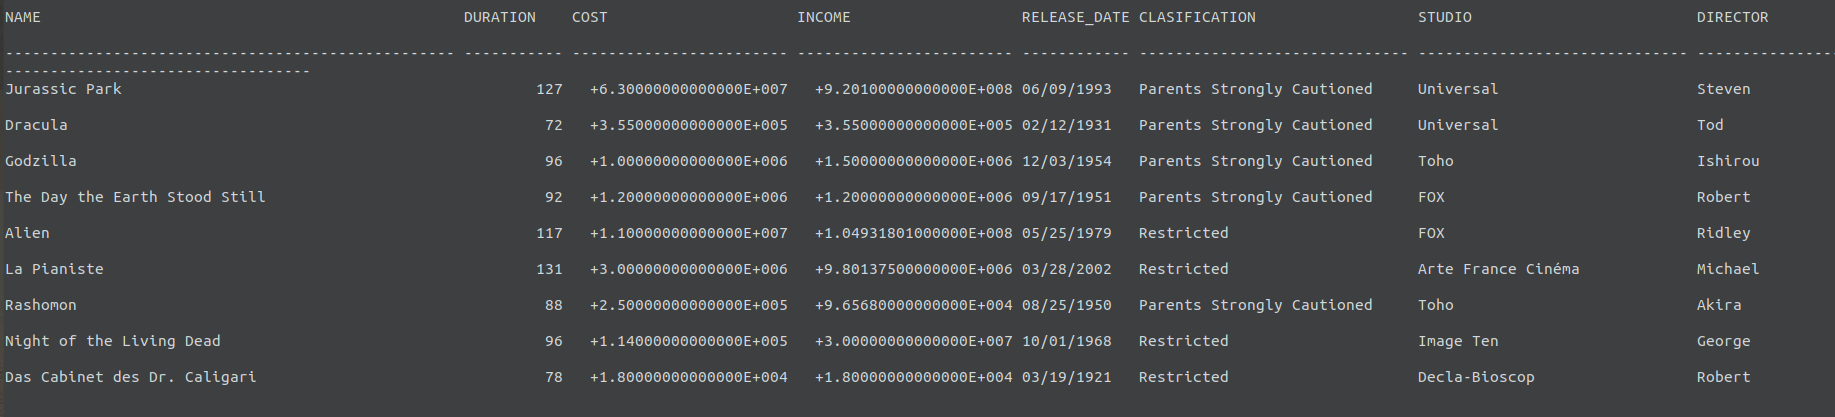
\includegraphics[scale=0.15]{figures/screenshot_vista3.png}
  	  	\caption{Vista de peliculas en base sus Ganancias.} \label{vista3}
\end{figure}
\end{frame}

\section{Index}

\begin{frame}[fragile]{Index}
Para agilizar el resultado de las peticiones a las vistas mencionadas se implementaron los siguientes \textit{Index}:

\begin{verbatim}
CREATE INDEX COUNTRY_ID 	ON MOVIEINDEX.COUNTRY(NAME);
CREATE INDEX INCOME 		ON MOVIEINDEX.MOVIE(INCOME);
CREATE INDEX COST			ON MOVIENDEX.MOVIE(COST);
CREATE INDEX MOVIE_INDEX	ON MOVIEINDEX.MOVIE(NAME);
\end{verbatim}

\end{frame}

\section{Store Procedures}
	
\begin{frame}{Store Procedures}
Se utilizaron 5 procedimientos almacenados:
\begin{itemize}
\item[1.] Un procedimietno carga los datos a la tabla que vincula a los actores a cada pelicula.
\item[2.] Un procedimiento carga los datos a la tabla que vincula a los generos con cada pelicula.
\item[3.] Un procedimiento generar una lista de las peliculas con sus generos.
\item[4.] Un procedimiento generar una lista de las peliculas con sus actores.
\item[5.] Un procedimiento para calcular las ganancias de las peliculas.
\end{itemize}

\end{frame}

\begin{frame}[fragile]{Store Procedures}
Procedimiento 1:
\begin{tiny}
\begin{verbatim}
CREATE or REPLACE PROCEDURE MOVIEINDEX.MOVIE_ACTOR ( IN MOVIENAME VARCHAR(50), IN ACTORNAME VARCHAR(50) )
LANGUAGE SQL
P1:BEGIN
    DECLARE ACTOR_ID int;
    DECLARE MOVIE_ID int;

    DECLARE cursor1 CURSOR FOR SELECT ID FROM MOVIEINDEX.MOVIE WHERE MOVIENAME = MOVIEINDEX.MOVIE.NAME;
    DECLARE cursor2 CURSOR FOR SELECT ID FROM MOVIEINDEX.ACTOR WHERE ACTORNAME = MOVIEINDEX.ACTOR.NAME;
    OPEN cursor1;
        FETCH FROM cursor1 INTO ACTOR_ID;
    CLOSE cursor1;
    OPEN cursor2;
        FETCH FROM cursor2 INTO MOVIE_ID;
    CLOSE cursor2;

    INSERT INTO MOVIEINDEX.ACTOR_MOVIE (ACTORDID, MOVIEDID) VALUES (ACTOR_ID, MOVIE_ID);
END P1
@
\end{verbatim}
\end{tiny}
\end{frame}

\begin{frame}[fragile]{Store Procedures}
Procedimiento 2:
\begin{tiny}
\begin{verbatim}
CREATE or REPLACE PROCEDURE MOVIEINDEX.MOVIE_GENDER ( IN MOVIENAME VARCHAR(50), IN GENDERNAME VARCHAR(50) )
LANGUAGE SQL
P1:BEGIN
  DECLARE GENDER_ID int;
  DECLARE MOVIE_ID int;

  DECLARE cursor1 CURSOR FOR SELECT ID FROM MOVIEINDEX.MOVIE WHERE MOVIENAME = MOVIEINDEX.MOVIE.NAME;
  DECLARE cursor2 CURSOR FOR SELECT ID FROM MOVIEINDEX.GENDER WHERE GENDERNAME = MOVIEINDEX.GENDER.NAME;
    OPEN cursor1;
        FETCH FROM cursor1 INTO GENDER_ID;
    CLOSE cursor1;
    OPEN cursor2;
        FETCH FROM cursor2 INTO MOVIE_ID;
    CLOSE cursor2;

    INSERT INTO MOVIEINDEX.GENDER_MOVIE (GENDERID, MOVIEID) VALUES (GENDER_ID, MOVIE_ID);
END P1
@
\end{verbatim}
\end{tiny}
\end{frame}

\begin{frame}[fragile]{Store Procedures}
Procedimiento 3:
\begin{tiny}
\begin{verbatim}
CREATE or REPLACE PROCEDURE MOVIEINDEX.GENDERS_PER_MOVIE ( IN MOVIENAME VARCHAR(50), OUT GENDERS INT )
LANGUAGE SQL
P5:BEGIN
    DECLARE MOVIEID int;

    DECLARE cursor1 CURSOR FOR SELECT ID FROM MOVIEINDEX.MOVIE WHERE MOVIEINDEX.MOVIE.NAME = MOVIENAME;
    OPEN cursor1;
        FETCH FROM cursor1 INTO MOVIEID;
    CLOSE cursor1;

    DECLARE cursor2 CURSOR FOR SELECT COUNT(*) AS GENDERS_IN FROM MOVIEINDEX.MOVIE, 
    MOVIEINDEX.GENDER_MOVIE, MOVIEINDEX.GENDER 
    WHERE MOVIEINDEX.MOVIE.ID = MOVIEID AND 
    MOVIEINDEX.GENDER_MOVIE.MOVIEDID = MOVIEID AND 
    MOVIEINDEX.GENDER.ID = MOVIEINDEX.GENDER_MOVIE.GENDERID;
    OPEN cursor2;
        FETCH FROM cursor2 INTO GENDERS;
    CLOSE cursor2;
END P5
@
\end{verbatim}
\end{tiny}
\end{frame}


\begin{frame}[fragile]{Store Procedures}
Procedimiento 4:
\begin{tiny}
\begin{verbatim}
CREATE or REPLACE PROCEDURE MOVIEINDEX.ACTOR_IN_MOVIE ( IN MOVIENAME VARCHAR(50), OUT ACTORS INT )
LANGUAGE SQL
P4:BEGIN
    DECLARE MOVIEID int;

    DECLARE cursor1 CURSOR FOR SELECT ID FROM MOVIEINDEX.MOVIE WHERE MOVIEINDEX.MOVIE.NAME = MOVIENAME;
    OPEN cursor1;
        FETCH FROM cursor1 INTO MOVIEID;
    CLOSE cursor1;

    DECLARE cursor2 CURSOR FOR SELECT COUNT(*) AS ACTORS_IN FROM MOVIEINDEX.MOVIE, 
    MOVIEINDEX.ACTOR_MOVIE, 
    MOVIEINDEX.ACTOR WHERE MOVIEINDEX.MOVIE.ID = MOVIEID AND 
    MOVIEINDEX.ACTOR_MOVIE.MOVIEDID = MOVIEID AND 
    MOVIEINDEX.ACTOR.ID = MOVIEINDEX.ACTOR_MOVIE.ACTORID;
    OPEN cursor2;
        FETCH FROM cursor2 INTO ACTORS;
    CLOSE cursor2;
END P4
@
\end{verbatim}
\end{tiny}
\end{frame}


\begin{frame}[fragile]{Store Procedures}
Procedimiento 5:
\begin{tiny}
\begin{verbatim}
CREATE or REPLACE PROCEDURE MOVIEINDEX.REVENUE ( IN MOVIENAME VARCHAR(50), OUT TOTAL FLOAT )
LANGUAGE SQL
P1:BEGIN

    DECLARE cursor1 CURSOR FOR SELECT SUM(INCOME - COST) AS MOVIEREVENUE FROM MOVIEINDEX.MOVIE WHERE MOVIENAME = MOVIEINDEX.MOVIE.NAME;
    OPEN cursor1;
        FETCH FROM cursor1 INTO TOTAL;
    CLOSE cursor1;
END P1
@
\end{verbatim}
\end{tiny}
\end{frame}

\section{A implementar}


\begin{frame}{Triggers}
\begin{itemize}
\item[1.]Log el usiario de cada insert
\item[2.]Cuando una pelicula salga de existencia el titulo se agrega a una vista de ``Request"

\end{itemize}

\end{frame}

\section{DDL}
\begin{frame}

\end{frame}
\end{document}
 